% !TEX root = ../MichaelsThesis.tex
%
\chapter{Introduction} \label{chapter1:introduction}
%
My journey in writing this thesis started with an interest in research in the biomedical engineering field. I participated in a summer REU (Research Experience for Undergraduates) at Penn State, my initial project that I was involved with was investigating  a computational model of blood under various flow conditions. After that summer, I started down the path to write this thesis in earnest. The mathematical model that describes the flood of blood has terms that are typical of advection, reaction, and diffusion problems. Among the many mathematical features of the blood model, two particular ones present some issues when solved numerically. The focus of this thesis shifted from the actual model to the problem features of the model. The two specific features that the blood model exhibits are advection behavior in flows and the inf-sup condition. These features are not specific to the model for blood. In fact they can be demonstrated separately in simple 1D examples that will be presented later in this chapter.


Advection behavior occurs when the gradient of a field, say $\phi$, is multiplied by a velocity as in the term $\nabla\phi\cdot\bv{v}$. This behavior can be seen in the Navier-Stokes equations. In the Navier-Stokes problem the advection term is $(\nabla\bv{v})\bv{v}$. The Navier-Stokes equations also exhibit the inf-sup condition. The inf-sup condition comes from constraints that are enforced through Lagrange multipliers. The Lagrange multiplier in the Navier-Stokes equations is the incompressibility equation \textit{i.e.} $\nabla\cdot\bv{v} = 0$. The term $det\,\tensor{B_{\kappa}}=1$ in the blood model is a similar constraint that results in the inf-sup condition.
%
\section{Advection-Dominated Flow}
In order to demonstrate the numerical difficulties that advection-dominated flows present, we will consider an example with both the finite difference method and the finite element method. Consider the 1D advection-diffusion BVP,
\begin{align}
    \label{1d advec}
    u\, \partial_{x}\phi &= k\, \partial_{xx}\phi
    \\
    \label{1d advec bc1}
    \phi\,(0) &= 0
    \\
    \label{1d advec bc2}
    \phi\,(L) &= 1
\end{align}
where $u$ is the given flow velocity and $k$ is the diffusivity of $\phi$. \textcolor{red}{Please define L.} We assume that both $u$ and $k$ are positive and constant. The exact solution to the BVP stated in Eqs.~\eqref{1d advec}--\eqref{1d advec bc2} is
\begin{equation}
    \phi= \frac{1-e^{\frac{Pe\,x}{L}}}{1-e^{Pe}},
\end{equation}
where $Pe$ is the global Peclet number ($Pe=u\,L/k$). We can also define an elemental Peclet number $\alpha$ as
\begin{equation}
    \alpha=\frac{u\,h}{2k},
\end{equation}
%%
\textcolor{red}{where $h$ is ?}
\begin{figure}
    \centering
    %\begin{subfigure}
        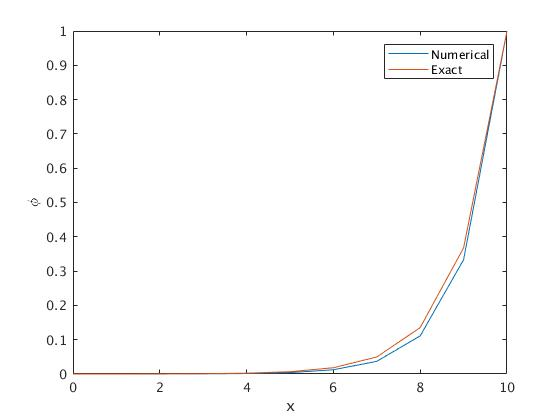
\includegraphics[width=0.3\textwidth]{Chapter-1/Figures/alpha_5}
        %\caption{$\alpha=0.5$}
      %  \label{fig:alpha=.5}
    %\end{subfigure}
    %\begin{subfigure}
       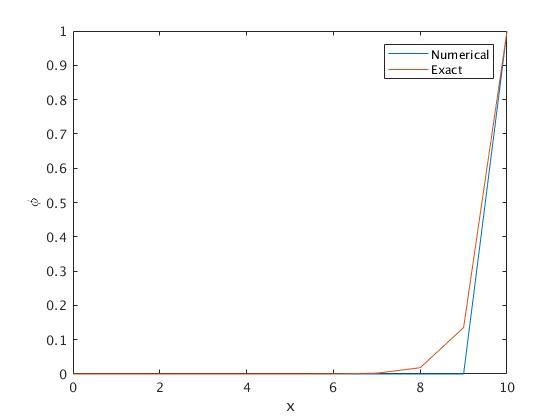
\includegraphics[width=0.3\textwidth]{Chapter-1/Figures/alpha1}
        %\caption{$\alpha=1$}
      %  \label{fig:alpha=1}
    %\end{subfigure}
    %\begin{subfigure}
        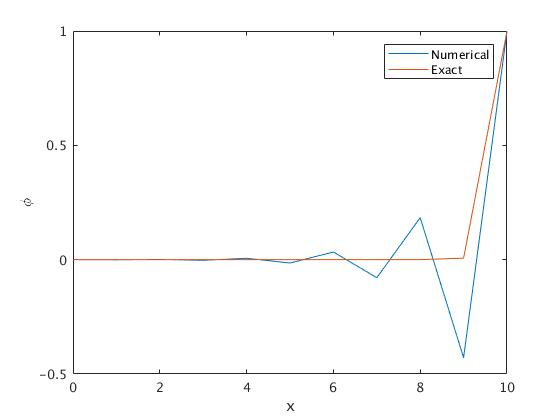
\includegraphics[width=0.3\textwidth]{Chapter-1/Figures/alpha2_5}
        % \caption{$\alpha=2.5$}
     %   \label{fig:alpha=2.5}
    %\end{subfigure}
\end{figure}